\documentclass[10.5pt]{beamer}

\usepackage[T1]{fontenc} 
\usepackage[utf8]{inputenc}
\usepackage{graphicx}
\usepackage{booktabs}
\usepackage[frenchb]{babel}
\usepackage{multirow}
\usepackage{subcaption}
\usepackage{float}
\usepackage{listings}

\usetheme{Warsaw}
\setbeamertemplate{navigation symbols}{}
\usecolortheme{beaver}
\addtobeamertemplate{footline}{\insertframenumber/\inserttotalframenumber}

\DeclareGraphicsExtensions{.jpeg,.jpg,.png}
%% \setbeamertemplate{itemize item}{\textcolor{red}{$\surd$}}
%% \newenvironment{proenv}{\only{\setbeamercolor{local structure}{fg=green}}}{}
%% \newenvironment{conenv}{\only{\setbeamercolor{local structure}{fg=red}}}{}
%%\item<conen@x->

%% \newcommand{\smiley}{\tikz[baseline=-0.75ex,black]{
%%     \draw circle (2mm);
%% \node[fill,circle,inner sep=0.5pt] (left eye) at (135:0.8mm) {};
%% \node[fill,circle,inner sep=0.5pt] (right eye) at (45:0.8mm) {};
%% \draw (-145:0.9mm) arc (-120:-60:1.5mm);
%%     }
%% }

%% \newcommand{\frownie}{\tikz[baseline=-0.75ex,black]{
%%     \draw circle (2mm);
%% \node[fill,circle,inner sep=0.5pt] (left eye) at (135:0.8mm) {};
%% \node[fill,circle,inner sep=0.5pt] (right eye) at (45:0.8mm) {};
%% \draw (-145:0.9mm) arc (120:60:1.5mm);
%%     }
%% }
%% \item[\smiley]

\title[Émulation d'applications distribuées]{Émulation d'applications distribuées \\ sur SimGrid via Simterpose}
\author{Louisa Bessad}
\institute{Université Pierre et Marie Curie \\
  \medskip
  \textit{louisa.bessad@gmail.com}}

\titlegraphic{
\includegraphics[scale=0.1]{Pictures/png/UPMC_sorbonne.png} \hspace{0.5cm}
  
\includegraphics[scale=0.07]{Pictures/loria_logo.jpg}}
\date{7 Septembre 2015}

\begin{document}

\begin{frame}[plain]
\titlepage
\end{frame}
\setbeamercovered{transparent}
\setbeamertemplate{navigation symbols}{\insertframenumber}
%------------------------------------------------
% Pourquoi l'émulation par interception
%------------------------------------------------
\section{Pourquoi l'émulation et quel type}
\subsection{Tester des applications distribuées}
\begin{frame}{\subsecname}

 \textbf{3 méthodes:}
  \begin{itemize}
  \item <1-> \textbf{Exécution sur plateforme réelle} (PlanetLab, Grid'5000)
    \begin{itemize}
    \item <1-> Étude du comportement en conditions réelles
    \item <1-> Lourd et difficilement reproductible
    \end{itemize}
    
    %%\setbeamercovered{transparent}{
    \item <2-> \textbf{Simulation} (SimGrid)
      
      Exécution d'un modèle de l'application
      \begin{itemize}
      \item <2-> Mise en \oe uvre simple et facilement reproductible
      \item <2-> Validation d'un modèle
      \end{itemize}
    %%}
  \item <3> \textbf{Émulation}
    
     Substitution de l'environnement par un logiciel
    \begin{itemize}
    \item <3> Exécution réelle dans un environnement virtuel
    \item <3> Une version de code
    \end{itemize}
     Emulation standard ou légère?
  \end{itemize}
  
%%  }
\end{frame}

\subsection{Types d'émulation légère}
\begin{frame}{\subsecname}
  \frametitle{Émulation légère par dégradation}
  \begin{columns}[c]
    \begin{column}{3cm}
        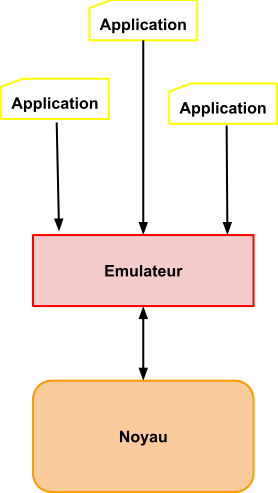
\includegraphics[scale=0.3]{Pictures/png/Virtualisation_limitation}    
    \end{column}
    \begin{column}{6cm}
        Simple à mettre en \oe uvre
        
        Dépend de la puissance de l'hôte

    \end{column}
  \end{columns}
\end{frame}

\begin{frame}{\subsecname}
  \frametitle{Émulation légère par interception}
  \begin{center}
    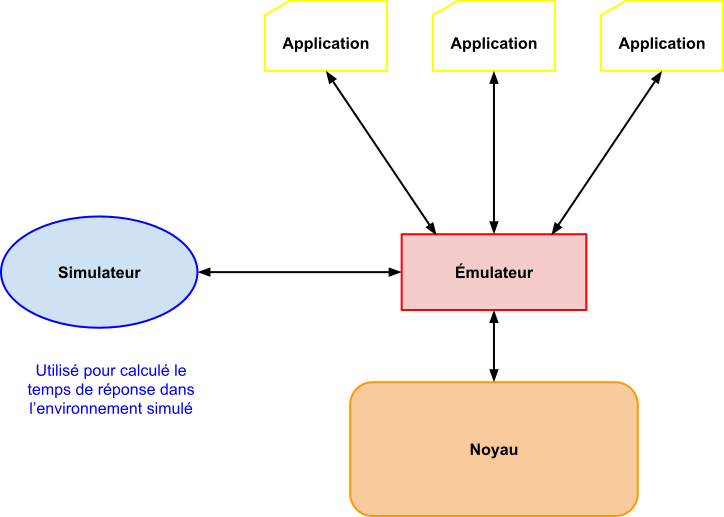
\includegraphics[scale=0.2]{Pictures/png/Virtualisation_interception}

    \vspace{0.5cm}
  \begin{minipage}{7cm}
  \begin{itemize}
  \item Simulateur: l'environnement virtuel
  \item Émulateur: Interception
  \end{itemize}
  \end{minipage}
  \end{center}
\end{frame}
%------------------------------------------------
% Notre projet
%------------------------------------------------ 
\section{SimGrid et Simterpose}
\subsection{Objectif}
\begin{frame}{\subsecname}
  
  \begin{alertblock}{Propriété de l'émulateur}
    \begin{itemize}
    \item Simple d'utilisation + facilement déployable
    \item Conditions expérimentales variées
    \item Expériences reproductibles 
    \item Résistance aux pannes et fautes
    \item Pas d'accès au fichier source
    \end{itemize}
  \end{alertblock}

  \begin{block}<2->{Choix}
    \begin{itemize}
  \item Émulation par interception
  \item Simulateur: SimGrid
  \item Émulateur: Simterpose
    \end{itemize}
  \end{block}
\end{frame}

\subsection{Organisation}
\begin{frame}{\secname}
  \centering
  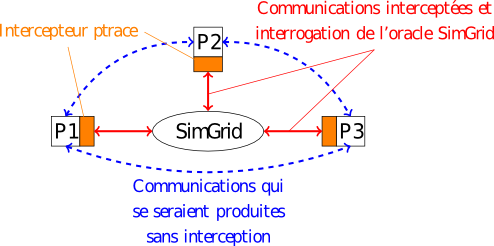
\includegraphics[scale=0.65]{Pictures/png/Communications_Simterpose_interprocess_v1}
\end{frame}

%------------------------------------------------
% Comment intercepter
%------------------------------------------------
\section{Outils d'interception}
\subsection{Niveaux d'interception}
\begin{frame}
  \frametitle{Actions à intercepter}
  \begin{columns}[c]
    \begin{column}{4cm}
      \begin{itemize}
      \item Communications réseau
      \item Temps
      \item Threads
      \item DNS
      \end{itemize}
    \end{column}
    \begin{column}{7cm}
        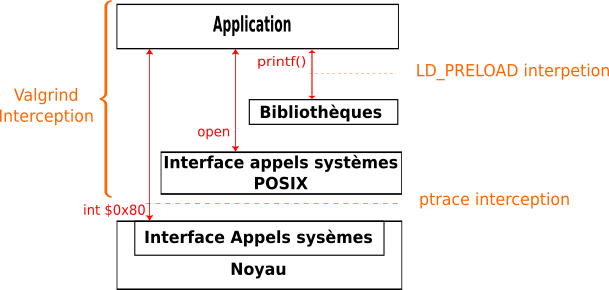
\includegraphics[scale=0.4]{Pictures/png/Communication_application_noyau_v3.png}<2->
  \end{column}
\end{columns}        
\end{frame}

\subsection{Haut niveau}
\begin{frame}{\subsecname}
  \begin{alertblock}{Binaire: Valgrind}
    \begin{itemize}
    \item Ré-écriture à la volée de fonctions à intercepter
    \item Temps d'exécution x 7.5
    \end{itemize}
  \end{alertblock}
  
  \begin{alertblock}<2->{Bibliothèques: \texttt{LD\_PRELOAD}}
    \begin{itemize}
    \item Variable d'environnement
    \item Permet de charger des bibliothèques dynamiques avant les autres
    \end{itemize}
  \end{alertblock}
\end{frame}

\subsection{Bas niveau: Appels Systèmes}
\begin{frame}{\subsecname}
  \begin{alertblock}{\texttt{ptrace}}
    \begin{itemize}
    \item Appel système qui permet de contrôler un processus
    \item<2-> Choix des actions de contrôle
    \item<3-> Modification des appels systèmes (handler et registres)
    \item<4-> Nombreux changements de contexte + Non POSIX
    \end{itemize}
  \end{alertblock}
\end{frame}
\begin{frame}{\subsecname}
  \begin{alertblock}{Uprobes}
    \begin{itemize}
    \item Insertion de points d'arrêt (API Noyau)
    \item Module noyau contient le handler de l'appele
    \item Évite les changements de contexte
      \item Rapide + accès à toutes les ressources
    \end{itemize}
  \end{alertblock}
    \begin{alertblock}<2->{seccomp/BPF}
  \begin{itemize}
  \item Choix des appels systèmes autorisés à s'exécuter
  \item Fait uniquement de l'interception
  \item Utilise \texttt{ptrace} pour modifier l'appel système
    \end{itemize}
    \end{alertblock}
\end{frame}

\subsection{Quels outils pour quelle interception}
\begin{frame}{\subsecname}
  \begin{columns}[c]
    \begin{column}{5cm}
      \begin{alertblock}{\texttt{ptrace}}
        \begin{itemize}
        \item Coût: Moyen
        \item Mise en \oe uvre: Complexe
        \item Utilisation: \\ Thread (partiel) + Réseau
        \end{itemize}
      \end{alertblock}
    \end{column}
    \begin{column}{5cm}
      \begin{alertblock}<2->{\texttt{LD\_PRELOAD}}
        \begin{itemize}
        \item Coût: Faible
        \item Mise en \oe uvre: Simple
        \item Utilisation: \\ Temps + Thread + DNS
        \end{itemize}
      \end{alertblock}
    \end{column}
  \end{columns}  

  \begin{alertblock}<3->{Implémentation}
    \begin{itemize}
    \item Réseau de communications: \texttt{ptrace}
    \item Temps: \texttt{LD\_PRELOAD}
    \item Thread: \texttt{ptrace} + \texttt{LD\_PRELOAD}
    \item DNS: \texttt{LD\_PRELOAD}
    \end{itemize}
  \end{alertblock}
\end{frame}
%------------------------------------------------
% Travail et résultats
%------------------------------------------------
\section{Travail réalisé, résultats, analyse}
\subsection{Réseau de communications et médiations}
\begin{frame}{\subsecname}
\begin{alertblock}{Vision du réseau}
 \begin{columns}[c]
   \begin{column}{4cm}
     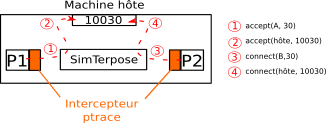
\includegraphics[scale=0.5]{Pictures/png/Mediation_realite}
   \end{column}
   \begin{column}{4cm}
      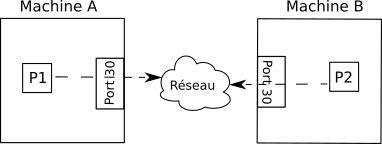
\includegraphics[scale=0.4]{Pictures/png/Mediation_VM}
   \end{column}
 \end{columns}
 
\end{alertblock}

 %%  \begin{figure}[H]
 %%   \centering
 %%   \begin{subfigure}{0.5\textwidth}
 %%   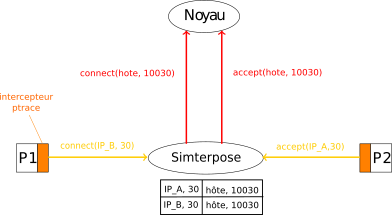
\includegraphics[scale=0.4]{Pictures/png/Mediation_translation_v2}
 %%   \caption{\textit{Address translation}}
 %%   \label{ADDRESS_TRANSLATION}
 %%   \end{subfigure}
 %%   \begin{subfigure}{0.4\textwidth}
 %%     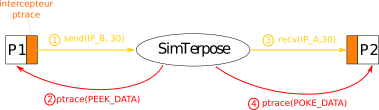
\includegraphics[scale=0.4]{Pictures/png/Mediation_full_v2}
 %%  \caption{\textit{Full mediation}}
 %%   \end{subfigure}
 %% \end{figure}
\begin{columns}[c]
  \begin{column}{5cm}
    \begin{block}<2->{Address Translation}
      \centering
      \includegraphics[scale=0.4]{Pictures/png/Mediation_translation_v2_pres}
    \end{block}
  \end{column}
  \begin{column}{5cm}
    \begin{block}<3->{Full Mediation}
      \centering
      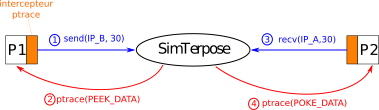
\includegraphics[scale=0.4]{Pictures/png/Mediation_full_v1_pres}
    \end{block}
  \end{column}
\end{columns}
\end{frame}

\begin{frame}{\subsecname}
  \frametitle{Overhead concernant le temps d'exécution}
  \begin{columns}[c]
    \begin{column}{4cm}
      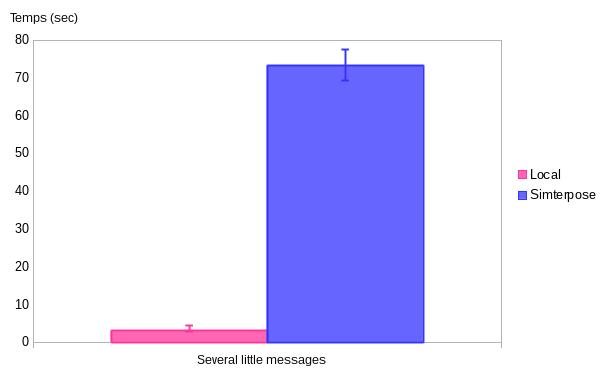
\includegraphics[scale=0.25]{mesures/graph/Littlemsg_local_pres.jpg}
    \end{column}
    \begin{column}{4cm}
      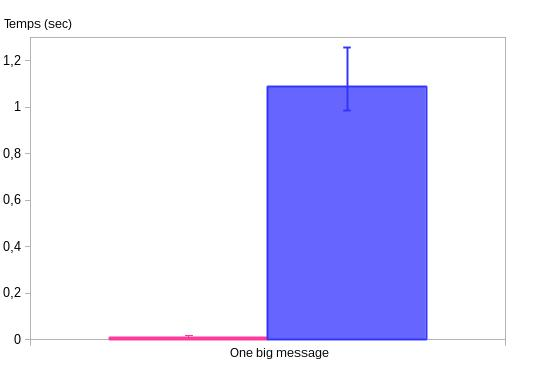
\includegraphics[scale=0.25]{mesures/graph/Bigmsg_local_pres.jpg}
     \end{column}
 \end{columns}

\begin{itemize}
\item Temps moyen d'exécution:
  \begin{itemize}
    \item Gros message: 0.01s en local, 1,05s avec Simterpose
    \item Petits messages: 3s en local, 73.5s avec Simterpose
  \end{itemize}
\item<2-> Analyse:
  \begin{itemize}
  \item<2-> Nombreux appels systèmes et changements de contexte
  \end{itemize}
\end{itemize}
\end{frame}

\begin{frame}
  \frametitle{Quelle médiation pour quel type d'application}
  \begin{columns}[c]
    \begin{column}{4cm} 
   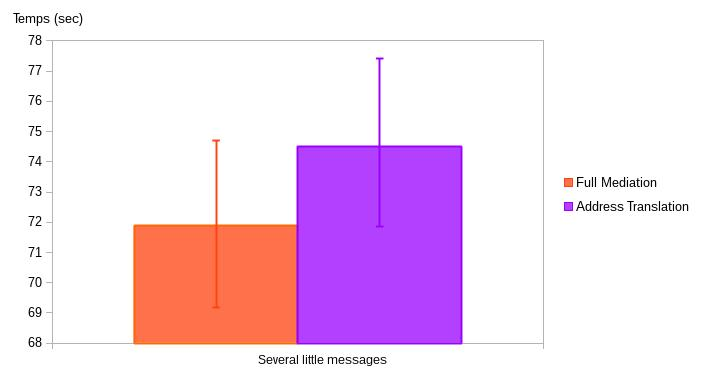
\includegraphics[scale=0.23]{mesures/graph/Littlemsg_pres.jpg}
   \end{column}
    \begin{column}{4cm}
   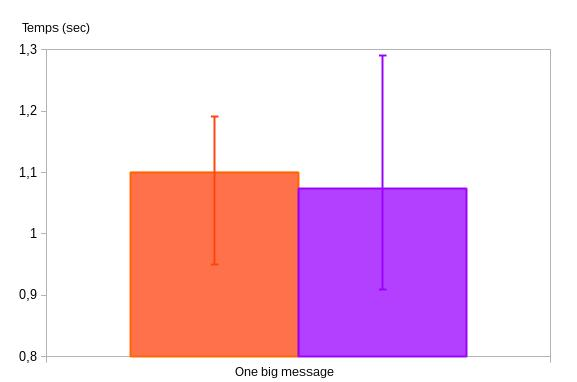
\includegraphics[scale=0.23]{mesures/graph/Bigmsg_pres.jpg}
    \end{column}
  \end{columns}
  
  \begin{itemize}
  \item Temps moyen d'exécution
    \begin{itemize}
    \item Gros message: Écart de 2.5\%
    \item Petits messages: Écart de 3\%
    \end{itemize}
  \item<2-> Analyse
    \begin{itemize}
    \item<2-> Petits messages: \textit{full mediation} plus rapide car aucun appel système exécuté
    \item<2-> Gros message: Gestion mémoire ralentie la \textit{full mediation}
    \end{itemize}
  \end{itemize}

\end{frame}

\subsection{Gestion du temps}
\begin{frame}{\subsecname}
  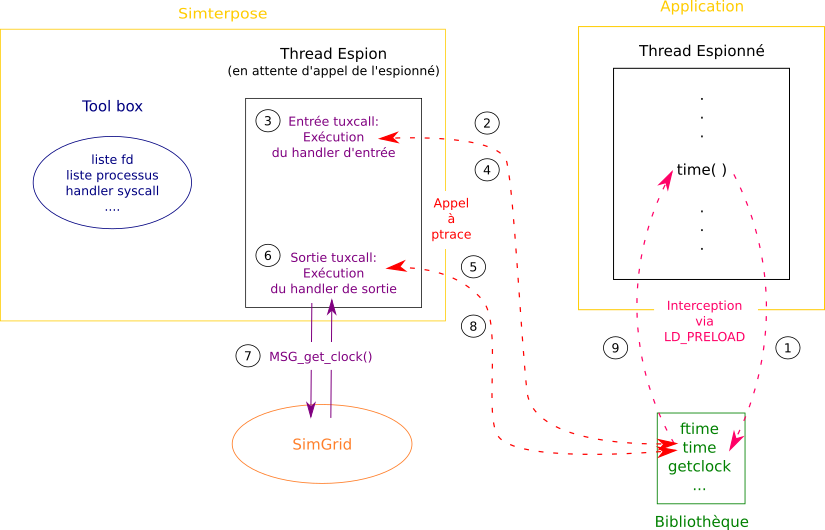
\includegraphics[scale=0.4]{Pictures/png/Open_pandor}
\end{frame}

\begin{frame}{\subsecname}
  
  %% \begin{columns}[c]
  %%   \begin{column}{5cm}
  \centering
      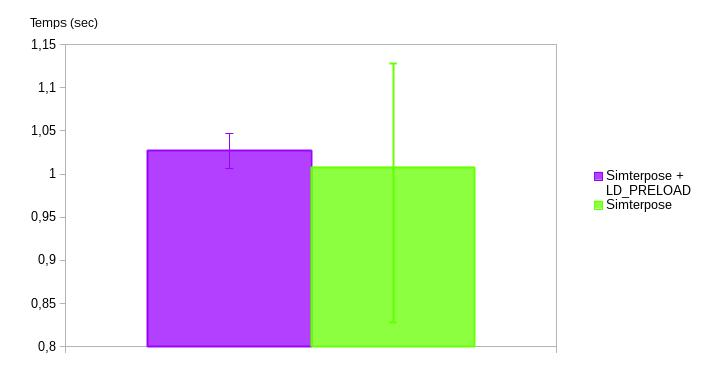
\includegraphics[scale=0.25]{mesures/graph/global_time.jpg}
    %% \end{column}
    %% \begin{column}{4cm}
      \begin{itemize}
      \item Temps moyen d'exécution
        \begin{itemize}
        \item Sans interception: 1s
        \item Avec interception: 1.02s 
        \end{itemize}
    %%   \end{itemize}
  %%   \end{column}
  %% \end{columns}
  
  %% \begin{itemize}
  \item<2-> Analyse
    \begin{itemize}
    \item<2-> Appel à la bibliothèque \texttt{VDSO} sans interception coûteuse en accès mémoire
    \end{itemize}
  \end{itemize}
\end{frame}

\subsection{Améliorations}
\begin{frame}{\subsecname}
  \begin{itemize}
  \item Portabilité de Simterpose sur des architectures 32 bits
  \item<2-> Mise à niveau de la version de SimGrid utilisée
  \item<3-> Création d'un système de fichiers pour Simterpose
  \item<4-> Utilisation de Valgrind possible
    \end{itemize}
\end{frame}

%------------------------------------------------
% Conclusions + Future Works
%------------------------------------------------
\section{Conclusions et perspectives}
\begin{frame}
  \frametitle{Pour finir}
  \begin{alertblock}{Conclusions}
    \begin{itemize}
    \item 2 fonctionnalités implémentées
    \item Virtualisation possible pour les 2 fonctionnalités
    \item Améliorations apportées
    \end{itemize}
  \end{alertblock}
  \begin{alertblock}<2->{Perspectives}
    \begin{itemize}
    \item 2 fonctionnalités restantes
    \item Troisième type de médiation ``accès direct''
    \item Nouvelles expériences
      \begin{itemize}
      \item Influence du nombre de processus sur les performances et la mémoire
      \item Tirage aléatoire des tailles de messages
      \item Exécution avec BitTorrent
      \end{itemize}
    \end{itemize}
  \end{alertblock}
\end{frame}

\setbeamertemplate{navigation symbols}{}
%------------------------------------------------
% Annexe
%------------------------------------------------
\defverbatim[colored]\lstI{
\begin{lstlisting}[language=bash,basicstyle=\ttfamily,keywordstyle=\color{red},commentstyle=\itshape\color{green!40!black}, breaklines=true,basicstyle=\footnotesize\ttfamily]
  > sudo simterpose -s platform.xml deploiement.xml
  > sudo LD_PRELOAD=lib.so -s platform.xml deploiement.xml
  > sudo simterpose ``gdb --args'' -s platform.xml
    deploiement.xml
  > sudo simterpose valgrind -s platform.xml deploiement.xml
\end{lstlisting}
}

\begin{frame}[plain]
  \frametitle{Annexe: Utilisation de Simterpose}
  \begin{itemize}
  \item Pour une exécution simple (avec interception réseau uniquement) \\ \texttt{> sudo simterpose -s platform.xml deploiement.xml}
  \item Pour une exécution avec en plus l'interception du temps \\ \texttt{> sudo LD\_PRELOAD=lib.so -s platform.xml deploiement.xml}
  \item Pour utiliser un débogueur \\ \texttt{> sudo simterpose ``gdb --args'' -s platform.xml deploiement.xml}\\ \texttt{> sudo simterpose valgrind -s platform.xml deploiement.xml}
  \end{itemize}
\end{frame}

\defverbatim[colored]\lstB{
\begin{lstlisting}[language=C,basicstyle=\ttfamily,keywordstyle=\color{red},commentstyle=\itshape\color{green!40!black}, breaklines=true,basicstyle=\footnotesize\ttfamily]
  /* Macro to ask the clock to SimGrid */
  #define get_simulation_time(clock) \
  syscall(SYS_tuxcall, clock)

  /* Time function */
  time_t time(time_t *t){
    double* sec = (double *) malloc(sizeof(double));
    get_simulation_time(sec);
    if (t != NULL)
    t = (time_t *) sec;  
    return (time_t)(*sec);    
  }
   \end{lstlisting}
}

 \begin{frame}[plain]
   \frametitle{Annexe: Interception temporelle}
   \lstB
 \end{frame}

 \defverbatim[colored]\lstC{
\begin{lstlisting}[language=C,basicstyle=\ttfamily,keywordstyle=\color{red},commentstyle=\itshape\color{green!40!black},breaklines=true,basicstyle=\footnotesize\ttfamily]
  void syscall_tuxcall(reg_s * reg, process_descriptor_t * proc){
    if (proc_entering(proc))
    proc_inside(proc); /* syscall_tuxcall_enter */
    else
    syscall_tuxcall_post(reg, proc);  /* syscall_tuxcall_exit */
  }
  
  void syscall_tuxcall_post(reg_s * reg, process_descriptor_t * proc){
    proc_outside(proc);
    XBT_DEBUG("tuxcall_post");
     /* Ask the clock to SimGrid */
    double clock = MSG_get_clock(); 
    
    /* Put the return value in argument register of the syscall */
    ptrace_poke(proc->pid, (void *) reg->arg[1], &clock, sizeof(double)); 
  }
  \end{lstlisting}
} 
 \begin{frame}[plain]
   \frametitle{Annexe: Interception temporelle}
   \lstC
 \end{frame}
 
 \begin{frame}[plain]
   \centering
   \frametitle{Architecture de SimGrid}
   \centering
   \includegraphics[scale=0.5]{Pictures/png/SimGrid}
   \end{frame}
\end{document}
